\documentclass[conference]{IEEEtran}
\IEEEoverridecommandlockouts
% The preceding line is only needed to identify funding in the first footnote. If that is unneeded, please comment it out.
\usepackage{cite}
\usepackage{amsmath,amssymb,amsfonts}
\usepackage{algorithmic}
\usepackage{graphicx}
\usepackage{textcomp}
\usepackage{xcolor}
\usepackage{newunicodechar}
\newunicodechar{−}{-}
\def\BibTeX{{\rm B\kern-.05em{\sc i\kern-.025em b}\kern-.08em
    T\kern-.1667em\lower.7ex\hbox{E}\kern-.125emX}}
\begin{document}

\title{Noise-Trained Pseudo-Invertible Autoencoder for Calibration-Free Spectrum Sensing\\
}

\author{\IEEEauthorblockN{1\textsuperscript{st} Jessica Kamman}
\IEEEauthorblockA{\textit{Stevens Institute of Technology} \\
Hoboken, NJ USA \\
jkamman@stevens.edu}
\and
\IEEEauthorblockN{2\textsuperscript{nd}Cristina Comaniciu}
\IEEEauthorblockA{\textit{Stevens Institute of Technology} \\
\textit{Electrical and Computer Engineering}\\
Hoboken, NJ USA \\
ccomaniciu@stevens.edu}

}
\maketitle

\begin{abstract}
Reliable spectrum sensing is difficult at low signal-to-noise ratio
(SNR), particularly when the primary-user waveform and receiver noise
power are unknown. This paper presents Psi-NN, a noise-trained
pseudo-invertible convolutional autoencoder for blind spectrum sensing.
Each decoder layer is determined by the pseudoinverse of its
corresponding encoder layer, reducing the number of independently
trained parameters and constraining the reconstruction. Psi-NN is
trained only on noise and operates on normalized observation blocks,
requiring neither primary-user signal examples nor an explicit estimate
of the noise power. Signal activity is detected using the coefficient
of determination between each input and its reconstruction. Pulse
shaping and oversampling introduce temporal correlation, causing
signal-containing blocks to produce higher reconstruction scores than
white noise. At a measured false-alarm probability near $0.01$, Psi-NN
outperforms energy detection, MME, CAV, and a conventional autoencoder
at SNRs of $-10$ dB and below. At $-10$ dB, Psi-NN achieves
$P_d=0.80$, compared with $0.77$ for the strongest classical baseline
and $0.39$ for the conventional autoencoder.
\end{abstract}

\begin{IEEEkeywords}
spectrum sensing, cognitive radio, autoencoder, one-class learning,
pseudo-inverse, anomaly detection
\end{IEEEkeywords}

\section{Introduction}

Reliable spectrum sensing is essential in cognitive radio. Before
transmitting, a secondary user must determine whether a band is
occupied by a primary user. A missed detection may cause harmful
interference, whereas a false alarm prevents the secondary user from
using an available channel. This decision is particularly difficult
when distance or shadowing weakens the primary-user signal, requiring
reliable detection at SNRs below $-10$ dB.

Energy detection~\cite{b1,b7} requires no knowledge of the
primary-user waveform and has low computational complexity. Its
threshold, however, depends on the receiver noise power. Under even
modest noise-power uncertainty, energy detection exhibits an SNR wall
below which increasing the observation length does not restore
reliable detection~\cite{b7}. MME~\cite{b3} and CAV~\cite{b4} avoid
an explicit noise-power estimate by exploiting the temporal correlation
introduced by pulse shaping and oversampling. They therefore provide
important classical benchmarks for blind spectrum sensing.

Most deep-learning spectrum-sensing methods use supervised training
with labeled primary-user signals~\cite{b5}. Their performance may
depend on whether the signal types encountered during operation were
represented during training. One-class methods avoid this requirement.
Pablos \emph{et al.}~\cite{b2} trained a one-dimensional convolutional
autoencoder only on noise and treated signals as anomalies. With noise
captured by a software-defined radio, they observed poorer
reconstruction when a signal was present. Under the AWGN and per-block
normalization model used here, signal-containing blocks instead produce
higher reconstruction scores. Pulse-shaped signals contain temporal
structure that is absent from white noise, allowing the convolutional
network to reconstruct them more accurately.

This paper proposes Psi-NN, a pseudo-invertible convolutional
autoencoder in which each decoder layer is determined by the
Moore--Penrose pseudoinverse of its corresponding encoder
layer~\cite{b8}. The model is trained only on noise and requires neither
labeled primary-user signals nor an explicit estimate of the noise
power. Its reconstruction statistic acts as a scale-invariant,
correlation-based detector. At a measured false-alarm probability near
$0.01$, Psi-NN is compared with energy detection, MME, CAV, and a
conventional autoencoder. The results show the largest gain at SNRs of
$-10$ dB and below, while a matched decoder ablation supports the role
of the pseudoinverse constraint.

\section{System Model}
The system consists of a single-node spectrum-sensing receiver that determines whether a signal is present in an observed channel. The sensing problem is formulated as the binary hypothesis test
\begin{equation}
\begin{aligned}
\mathcal{H}_0 &: \quad y[n] = w[n],\\
\mathcal{H}_1 &: \quad y[n] = s[n] + w[n],
\end{aligned}
\qquad n=0,\ldots,N-1,
\label{eq:hypotheses}
\end{equation}
where $s[n]$ denotes the transmitted signal and $w[n]$ is additive white Gaussian noise. Each real noise component follows $\mathcal{N}(0,1)$, resulting in a fixed noise floor. Each observation contains $N=1024$ samples, and only the in-phase component is provided to the detectors.

The transmitted signals use BPSK, QPSK, 16-QAM, or cross 32-QAM modulation. Raised-cosine pulse shaping is applied with a roll-off factor of $0.35$. All modulation formats use the same sampling rate, with four samples per symbol in the main experiments. A random timing offset is applied to each observation so that the beginning of a block is not consistently aligned with a symbol boundary. Samples affected by the pulse-shaping filter's start-up transient are discarded.

The signal-to-noise ratio is defined as
\begin{equation}
\mathrm{SNR} = \frac{P_s}{\sigma_w^2},
\label{eq:snr}
\end{equation}
where $P_s$ is the signal power and $\sigma_w^2$ is the noise variance. For each signal-containing block, the SNR is drawn uniformly from a range of $\pm 2$ dB around its nominal value. Because the noise floor remains fixed, this variation represents SNR uncertainty. Noise-power uncertainty is modeled separately for the energy-detector baseline.

Each observation supplied to the learned and covariance-based detectors is independently standardized according to
\begin{equation}
x[n] = \frac{y[n]-\bar{y}}{\hat{\sigma}_y},
\label{eq:block_normalization}
\end{equation}
where $\bar{y}$ and $\hat{\sigma}_y$ are the sample mean and sample standard deviation of the observation block, respectively. This normalization removes block-level mean and scale information, requiring the detectors to identify structural characteristics of the received waveform. The energy detector operates on the unnormalized samples because its test statistic depends directly on the received energy.

Detector thresholds are selected using the Neyman--Pearson criterion. Each threshold is estimated from an independent, held-out set of noise-only observations to target a false-alarm probability of
\begin{equation}
P_{\mathrm{fa}}
=
\Pr\!\left(
\text{decide } \mathcal{H}_1
\mid
\mathcal{H}_0
\right)
=
0.01.
\label{eq:pfa}
\end{equation}

Detection performance is measured by
\begin{equation}
P_d
=
\Pr\!\left(
\text{decide } \mathcal{H}_1
\mid
\mathcal{H}_1
\right).
\label{eq:pd}
\end{equation}

The objective is to maximize $P_d$ while maintaining the target $P_{\mathrm{fa}}$. The present study considers sensing at a single receiver. Hidden-terminal conditions require observations from multiple receivers and are therefore left to cooperative spectrum sensing, as discussed in Section~V.

\section{Pseudo-Invertible Detector}
\label{sec:proposed_method}

\subsection{Reconstruction Statistic}
\label{subsec:reconstruction_statistic}
Let $\mathbf{x}\in\mathbb{R}^{N}$ denote a normalized observation block and let $\hat{\mathbf{x}}$ denote its reconstruction. Detection is based on the coefficient of determination
\begin{equation}
\beta
=
1-
\frac{
\left\lVert \mathbf{x}-\hat{\mathbf{x}}\right\rVert_2^2
}{
\left\lVert \mathbf{x}-\bar{x}\mathbf{1}\right\rVert_2^2
},
\label{eq:beta_statistic}
\end{equation}
where $\bar{x}$ is the sample mean of the observation and $\mathbf{1}$ is an all-ones vector of length $N$. The numerator is the reconstruction error, while the denominator is the total variation within the observation block. Thus, $\beta$ represents the fraction of the block variance explained by the reconstruction. A larger value indicates that the network has preserved more of the structure in the input.

The detector uses the decision rule
\begin{equation}
\beta
\mathop{\gtrless}_{\mathcal{H}_0}^{\mathcal{H}_1}
\gamma,
\label{eq:beta_decision_rule}
\end{equation}
where $\gamma$ is selected to satisfy the desired false-alarm probability. Consequently, the receiver decides $\mathcal{H}_1$ when $\beta>\gamma$.

\subsection{Pseudo-Invertible Architecture}
\label{subsec:psinn_architecture}

Psi-NN constrains each decoder layer to be the pseudoinverse of its
corresponding encoder layer. If an encoder applies the linear operator
$\mathbf{W}$, the decoder applies its right Moore-Penrose pseudoinverse,
\begin{equation}
\mathbf{W}^{+}
=
\mathbf{W}^{\mathsf{T}}
\left(
\mathbf{W}\mathbf{W}^{\mathsf{T}}
\right)^{-1}.
\label{eq:right_pseudoinverse}
\end{equation}
This expression assumes that $\mathbf{W}$ has full row rank. Because
the decoder operator is computed directly from the encoder, its weights
are not learned independently. The reconstruction is therefore
constrained by the representation learned by the encoder.

The encoder contains three one-dimensional strided convolutional
layers. Each layer uses a kernel size of five and a stride of two, with
channel dimensions
\begin{equation}
1\rightarrow16\rightarrow64\rightarrow128.
\label{eq:psinn_channels}
\end{equation}
Batch normalization and a leaky rectified linear unit with negative
slope $0.2$ follow each convolution. Psi-NN contains $46{,}736$
trainable parameters, compared with $52{,}977$ for the Pablos CAE
baseline. The matched conventional autoencoder used in the decoder
ablation is described separately in
Section~\ref{subsec:decoder_ablation_results}.

The model is trained only on noise by minimizing the mean-squared
reconstruction error
\begin{equation}
\mathcal{L}_{\mathrm{MSE}}
=
\frac{1}{M}
\sum_{i=1}^{M}
\frac{1}{N}
\left\lVert
\mathbf{x}^{(i)}
-
\hat{\mathbf{x}}^{(i)}
\right\rVert_2^2,
\label{eq:training_mse}
\end{equation}
where $M$ is the number of training blocks and $N$ is the number of
samples in each block. No primary-user signals or modulation labels
are used during training.

The saved Psi-NN checkpoint was trained on $20{,}000$ noise-only
blocks using Adam with an initial learning rate of $10^{-3}$, a batch
size of 256, and 200 epochs. A StepLR schedule reduced the learning
rate by a factor of $0.5$ every 50 epochs. The reported checkpoint is
the model saved after the final epoch. The Pablos CAE followed its
separate reference training procedure: SGD with learning rate $0.02$,
a batch size of 256, and 50 epochs using a 90/10 training--validation
split. Its checkpoint was selected by the lowest validation loss.
These pretrained models were held fixed for every evaluation.

\subsection{Detection Mechanism}
\label{subsec:detection_mechanism}
Although Psi-NN is trained only to reconstruct noise, pulse-shaped signals produce larger values of $\beta$ than noise-only observations. The convolutional filters retain the temporal structure introduced by pulse shaping and oversampling more effectively than they retain uncorrelated white-noise fluctuations. Signal presence is therefore associated with a higher reconstruction score.

Figure~\ref{fig:beta_pdf_minus6db} shows the estimated distributions of $\beta$ under $\mathcal{H}_0$ and $\mathcal{H}_1$ at $-6$ dB. The signal-containing distribution is shifted toward larger values of $\beta$, indicating that Psi-NN reconstructs the structured signal component more accurately than white noise. Signal presence is therefore detected using the upper-tail rule $\beta>\gamma$. This decision direction is opposite to that reported by Pablos \emph{et al.}, who associated signal presence with poorer reconstruction.

\begin{figure}[t]
    \centering
    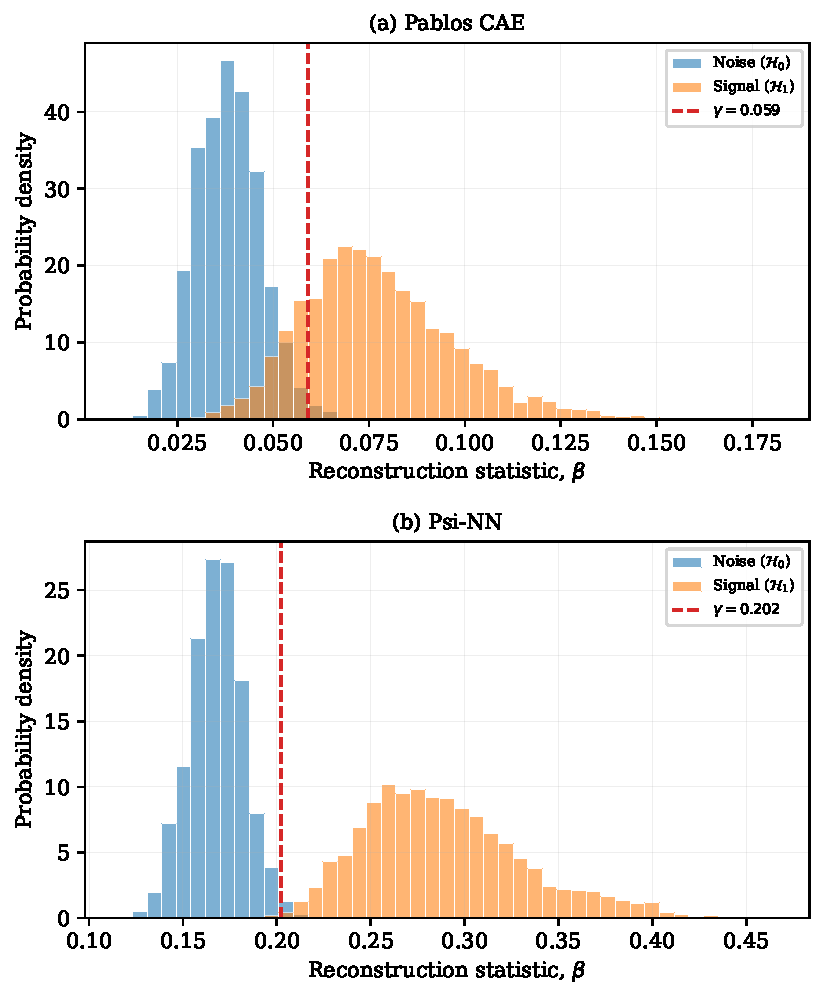
\includegraphics[width=\columnwidth]{figures/beta_pdf_minus6db.pdf}
    \caption{Estimated probability density of the reconstruction statistic
    $\beta$ under $\mathcal{H}_0$ and $\mathcal{H}_1$ at an SNR of $-6$ dB.
    The vertical line indicates the threshold $\gamma$ for
    $P_{\mathrm{fa}}=0.01$.}
    \label{fig:beta_pdf_minus6db}
\end{figure}

Per-block normalization also makes the statistic insensitive to a common change in input scale. If an observation is multiplied by a positive constant $a$, then

\begin{equation}
\frac{a\mathbf{y}-a\bar{y}}
     {a\hat{\sigma}_y}
=
\frac{\mathbf{y}-\bar{y}}
     {\hat{\sigma}_y}.
\label{eq:scale_invariance}
\end{equation}
The normalized input is therefore unchanged by the unknown scale factor. Detection performance also depends on the temporal correlation of the received signal. Oversampling and pulse shaping introduce structure across neighboring samples, allowing the convolutional network to distinguish signal-containing blocks from white noise. When this correlation is absent, the normalized signal becomes more noise-like and detection performance decreases.

\subsection{Threshold Selection}
\label{subsec:threshold_selection}
The threshold is determined from an independent calibration set containing noise-only observations. Let
\begin{equation}
\boldsymbol{\beta}_{\mathrm{cal}}
=
\left\{
\beta_{\mathrm{cal}}^{(1)},
\ldots,
\beta_{\mathrm{cal}}^{(M_{\mathrm{cal}})}
\right\}
\label{eq:calibration_scores}
\end{equation}
denote the reconstruction scores obtained from the calibration blocks. For an upper-tail detector, the threshold is the empirical $(1-P_{\mathrm{fa}})$ quantile,
\begin{equation}
\gamma
=
Q_{1-P_{\mathrm{fa}}}
\left(
\boldsymbol{\beta}_{\mathrm{cal}}
\right),
\label{eq:empirical_gamma}
\end{equation}
where $Q_q(\cdot)$ denotes the empirical $q$th quantile. With the operating point used in this work,
\begin{equation}
\gamma
=
Q_{0.99}
\left(
\boldsymbol{\beta}_{\mathrm{cal}}
\right).
\label{eq:gamma_001}
\end{equation}

The calibration observations are separate from both the training set and the final test set. This prevents the threshold from being fitted to the training noise and allows the false-alarm probability to be measured independently on held-out test observations.

\section{Results}
\label{sec:results}
\subsection{Experimental Setup}
\label{subsec:experimental_setup}

The main experiment used four samples per symbol and $N=1024$ samples
per observation. At each nominal SNR, the test set contained $1{,}000$
blocks for each of four modulations, giving $4{,}000$ signal-present
observations. The SNR ranged from $-14$ to $10$ dB in steps of $2$ dB,
with an independent uniform $\pm2$-dB variation applied to each
signal-present block.

The test set contained $1{,}000$ noise-only blocks at each SNR index,
or $13{,}000$ in total. Thresholds were estimated using a separate set
of $10{,}000$ noise blocks. Psi-NN and the CAE produced measured
false-alarm probabilities of $0.0108$; the MME, CAV, and known-noise
energy-detector results ranged from $0.0092$ to $0.0109$. The
uncertainty-aware energy detector was intentionally conservative and
produced approximately zero false alarms under nominal noise.

\subsection{Baseline Detectors}
\label{subsec:baseline_detectors}

The known-noise energy detector uses
\begin{equation}
T_{\mathrm{ED}}
=
\sum_{n=0}^{N-1}y^2[n].
\label{eq:ed_statistic_results}
\end{equation}
Its threshold was obtained from held-out noise. For the $\pm2$-dB
noise-uncertainty variant, the threshold was multiplied by
$10^{2/10}=10^{0.2}$.

MME and CAV were calculated from the $L\times L$ lag-covariance matrix
$\mathbf{R}_y$:
\begin{equation}
T_{\mathrm{MME}}
=
\frac{\lambda_{\max}(\mathbf{R}_y)}
     {\lambda_{\min}(\mathbf{R}_y)}
\label{eq:mme_statistic_results}
\end{equation}
and
\begin{equation}
T_{\mathrm{CAV}}
=
\frac{\sum_{i=1}^{L}\sum_{j=1}^{L}
\left|[\mathbf{R}_y]_{ij}\right|}
{\sum_{i=1}^{L}\left|[\mathbf{R}_y]_{ii}\right|}.
\label{eq:cav_statistic_results}
\end{equation}
Both detectors were evaluated with $L\in\{4,8\}$, and the stronger
configuration was reported. The neural baseline used the
one-dimensional autoencoder of Pablos \emph{et al.}~\cite{b2}. Its
encoder follows the channel progression
$1\rightarrow16\rightarrow64\rightarrow128$, while its bottleneck
decoder uses
$128\rightarrow8\rightarrow8\rightarrow16\rightarrow1$. The model
contains $52{,}977$ trainable parameters.

All neural and covariance-based detectors used the same normalized
in-phase observations and held-out calibration noise. The energy
detectors used the corresponding unnormalized samples. Supervised
detectors were excluded because they require labeled primary-user
signals, whereas the methods compared here are blind or one-class.

\subsection{Main Detection Results}
\label{subsec:main_detection_results}
Fig.~\ref{fig:pd_sps_comparison} presents the detection curves for four
and eight samples per symbol. The main comparison uses four samples per
symbol and is shown in Fig.~\ref{fig:pd_sps_comparison}(a). Panel (b)
is discussed with the oversampling results in
Section~\ref{subsec:oversampling_results}. Only SNRs from $-14$ through
$-4$ dB are displayed because the leading detectors approach perfect
detection at higher SNRs.

\begin{figure}[!t]
    \centering
    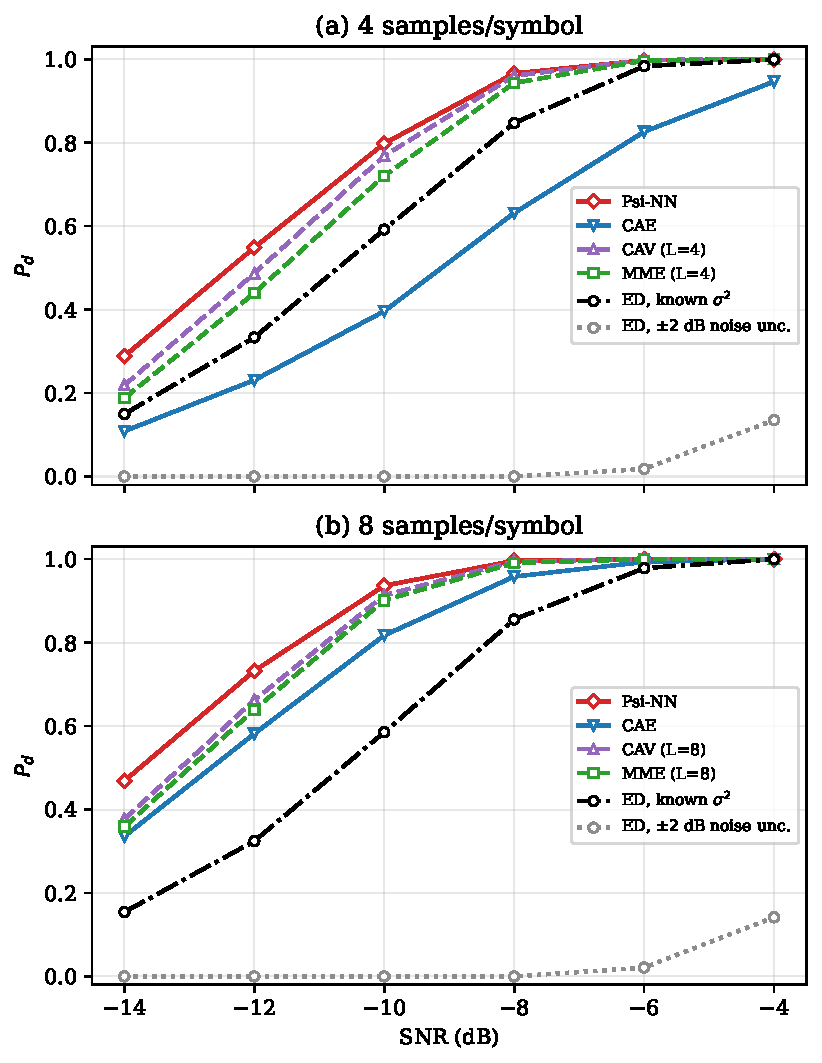
\includegraphics[
        width=0.98\columnwidth,
        keepaspectratio
    ]{figures/pd_vs_snr_4sps_8sps.pdf}
    \caption{Probability of detection versus nominal SNR for
    (a) four samples per symbol and (b) eight samples per symbol.
    The covariance dimensions are $L=4$ and $L=8$, respectively.
    All results use $P_{\mathrm{fa}}=0.01$.}
    \label{fig:pd_sps_comparison}
\end{figure}

Table~\ref{tab:main_pd_values} summarizes detection performance in the
low-SNR region. At $-14$, $-12$, and $-10$ dB, Psi-NN achieved the
highest detection probability among the evaluated detectors. At
$-14$ dB, Psi-NN achieved $P_d=0.289$, compared with $0.219$ for CAV,
$0.188$ for MME, $0.150$ for the known-noise energy detector, and
$0.109$ for the conventional autoencoder.

\begin{table}[!t]
\centering
\caption{Detection probability at four samples per symbol and
$P_{\mathrm{fa}}=0.01$.}
\label{tab:main_pd_values}
\resizebox{\columnwidth}{!}{%
\begin{tabular}{lcccc}
\hline
Detector & $-14$ dB & $-12$ dB & $-10$ dB & $-8$ dB \\
\hline
Psi-NN
    & \textbf{0.289} & \textbf{0.549}
    & \textbf{0.798} & \textbf{0.966} \\
CAV ($L=4$)
    & 0.219 & 0.487 & 0.769 & 0.960 \\
MME ($L=4$)
    & 0.188 & 0.440 & 0.721 & 0.943 \\
ED, known $\sigma^2$
    & 0.150 & 0.333 & 0.592 & 0.847 \\
CAE
    & 0.109 & 0.231 & 0.396 & 0.632 \\
ED, $\pm2$ dB uncertainty
    & 0.000 & 0.000 & 0.000 & 0.000 \\
\hline
\end{tabular}%
}
\end{table}

Psi-NN exceeded CAV by $0.070$, $0.062$, and $0.030$ at $-14$, $-12$,
and $-10$ dB, respectively. The corresponding bootstrap 95\%
confidence intervals were $[0.044,0.094]$, $[0.033,0.090]$, and
$[0.007,0.050]$, supporting the improvement at all three SNRs. At
$-8$ dB, the difference was $0.006$, with an interval of
$[-0.002,0.013]$; the detectors therefore cannot be clearly
distinguished once both approach reliable detection.

The gain from Psi-NN is thus concentrated at $-10$ dB and below, where
weak primary-user signals are most likely to be missed. In contrast,
the energy detector designed for $\pm2$-dB noise uncertainty produced
no detections through $-8$ dB and only $P_d=0.018$ at $-6$ dB,
illustrating its low-SNR wall.

Table~\ref{tab:modulation_results} separates the $-10$-dB results by
modulation. Each entry is based on $1{,}000$ signal-present blocks
generated at four samples per symbol. BPSK was comparatively easy for
all detectors. The separation was more demanding for QPSK, 16-QAM,
and cross 32-QAM because only the in-phase component was observed.
Psi-NN retained the highest detection probability for each of these
modulations, with its largest margin over CAV occurring for 32-QAM.

\begin{table}[!t]
\centering
\caption{Detection probability by modulation at $-10$ dB and four
samples per symbol.}
\label{tab:modulation_results}
\resizebox{\columnwidth}{!}{%
\begin{tabular}{lcccc}
\hline
Detector & BPSK & QPSK & 16-QAM & 32-QAM \\
\hline
Psi-NN
    & \textbf{0.987} & \textbf{0.742}
    & \textbf{0.734} & \textbf{0.729} \\
CAV ($L=4$)
    & 0.986 & 0.716 & 0.692 & 0.680 \\
MME ($L=4$)
    & 0.977 & 0.662 & 0.634 & 0.610 \\
ED, known $\sigma^2$
    & 0.915 & 0.489 & 0.494 & 0.469 \\
CAE
    & 0.679 & 0.296 & 0.292 & 0.318 \\
\hline
\end{tabular}%
}
\end{table}

\subsection{Effect of Oversampling}
\label{subsec:oversampling_results}


Fig.~\ref{fig:pd_sps_comparison}(b) and
Table~\ref{tab:oversampling_results} show the effect of sampling rate.
At $-10$ dB, Psi-NN increased from $P_d=0.302$ at two samples per
symbol to $0.798$ at four and $0.937$ at eight. CAV increased from
$0.425$ to $0.769$ and $0.914$, while MME increased from $0.434$ to
$0.721$ and $0.901$.

\begin{table}[!t]
\centering
\caption{Detection probability at $-10$ dB for different numbers of
samples per symbol. The target false-alarm probability is $0.01$.}
\label{tab:oversampling_results}
\resizebox{\columnwidth}{!}{%
\begin{tabular}{lccc}
\hline
Detector & 2 samples/symbol & 4 samples/symbol & 8 samples/symbol \\
\hline
Psi-NN
    & 0.302 & \textbf{0.798} & \textbf{0.937} \\
CAE
    & 0.086 & 0.396 & 0.818 \\
CAV
    & 0.425 & 0.769 & 0.914 \\
MME
    & 0.434 & 0.721 & 0.901 \\
ED, known $\sigma^2$
    & \textbf{0.609} & 0.592 & 0.585 \\
ED, $\pm2$ dB uncertainty
    & 0.000 & 0.000 & 0.000 \\
\hline
\end{tabular}%
}
\end{table}

At two samples per symbol, the known-noise energy detector performed
best, with $P_d=0.609$. In this setting, the sampled signal is nearly
white, leaving little temporal structure after normalization. As the
sampling rate increases, pulse shaping produces stronger correlation
between neighboring samples and improves Psi-NN, CAV, and MME. The
energy detector remains near $0.59$ because it depends on received
power rather than temporal correlation. These results support the
interpretation of Psi-NN as a learned correlation detector.

\subsection{Decoder Ablation}
\label{subsec:decoder_ablation_results}

Psi-NN was compared with a matched conventional autoencoder, denoted
Model~C, to isolate the effect of the pseudoinverse constraint. Both
models use the same in-phase input and encoder progression
$1\rightarrow16\rightarrow64\rightarrow128$. Psi-NN determines its
decoder from the encoder pseudoinverses, whereas Model~C uses an
independently trained symmetric decoder
$128\rightarrow64\rightarrow16\rightarrow1$. Model~C contains
$93{,}025$ trainable parameters.

Model~C is distinct from the $52{,}977$-parameter Pablos CAE used in
the main comparison. The Pablos CAE uses the bottleneck decoder
$128\rightarrow8\rightarrow8\rightarrow16\rightarrow1$, whereas
Model~C is included only as a conventional counterpart to the
pseudo-invertible decoder.

Both models were evaluated on the corrected four-sample test set using
empirical thresholds obtained from the same held-out calibration noise.
Their measured false-alarm probabilities were $0.0112$ for Model~C and
$0.0108$ for Psi-NN, placing both models near the target
$P_{\mathrm{fa}}=0.01$.

\begin{table}[!t]
\centering
\caption{Decoder ablation on the corrected four-sample test set.}
\label{tab:decoder_ablation}
\resizebox{\columnwidth}{!}{%
\begin{tabular}{lcccc}
\hline
Model & $-14$ dB & $-12$ dB & $-10$ dB & $-8$ dB \\
\hline
Matched conventional AE (Model C)
    & 0.073 & 0.169 & 0.296 & 0.519 \\
Psi-NN
    & \textbf{0.289} & \textbf{0.549}
    & \textbf{0.798} & \textbf{0.966} \\
\hline
\end{tabular}%
}
\end{table}

As shown in Table~\ref{tab:decoder_ablation}, Psi-NN exceeded Model~C
by $0.216$, $0.380$, and $0.502$ at $-14$, $-12$, and $-10$ dB,
respectively. Since the models share the same encoder dimensions and
were evaluated under the same testing and calibration conditions, the
results support the contribution of the pseudoinverse decoder
constraint to Psi-NN's low-SNR detection performance.

\subsection{Computational Complexity}
\label{subsec:complexity_results}

Psi-NN contains $46{,}736$ trainable parameters, compared with
$52{,}977$ for the Pablos CAE baseline. From the implemented layer
dimensions, one Psi-NN reconstruction requires $13{,}102{,}160$
convolutional MACs per block. This deployment-oriented count assumes
that the pseudoinverse matrices are cached after training; the current
research implementation recomputes them during each forward call.

The implemented CAV detector requires approximately $4{,}090$
lag-product MACs for $L=4$ and $8{,}164$ for $L=8$. Psi-NN therefore
requires roughly three orders of magnitude more computation. Its
benefit is concentrated at the lowest SNRs, where improved protection
of weak primary-user signals may justify the additional processing.

\section{Conclusion}
\label{sec:conclusion}

This paper presented Psi-NN, a noise-trained pseudo-invertible
autoencoder for blind spectrum sensing. Psi-NN requires neither
primary-user signal examples nor an explicit estimate of the noise
power. At a measured false-alarm probability near $0.01$, it achieved
detection probabilities of $0.289$, $0.549$, and $0.798$ at $-14$,
$-12$, and $-10$ dB, respectively, outperforming the evaluated
classical and neural baselines. The decoder ablation further showed
that the pseudoinverse constraint contributes to this low-SNR gain.

The oversampling results indicate that Psi-NN detects temporal
correlation introduced by pulse shaping. At $-10$ dB, its detection
probability increased from $0.302$ at two samples per symbol to $0.937$
at eight samples per symbol. This improvement comes at a higher
computational cost than CAV, making Psi-NN most useful when protecting
weak primary-user signals justifies the additional processing. Future
work will consider over-the-air measurements, hardware nonlinearities,
and cooperative sensing for hidden-terminal conditions.










\begin{thebibliography}{00}
\bibitem{b1} H. Urkowitz, ``Energy detection of unknown deterministic
signals,'' \textit{Proc. IEEE}, vol. 55, no. 4, pp. 523--531, Apr. 1967.
\bibitem{b2} C. Pablos, \'{A}. G. Andrade, and G. Galaviz,
``Modulation-Agnostic Spectrum Sensing based on Anomaly Detection for
Cognitive Radio,'' \textit{ICT Express}, vol. 9, no. 3, pp. 398--402,
Jun. 2023.
\bibitem{b3} Y. Zeng and Y.-C. Liang, ``Eigenvalue-based spectrum
sensing algorithms for cognitive radio,'' \textit{IEEE Trans. Commun.},
vol. 57, no. 6, pp. 1784--1793, Jun. 2009.
\bibitem{b4} Y. Zeng and Y.-C. Liang, ``Spectrum-sensing algorithms for
cognitive radio based on statistical covariances,'' \textit{IEEE Trans.
Veh. Technol.}, vol. 58, no. 4, pp. 1804--1815, May 2009.
\bibitem{b5} J. Gao, X. Yi, C. Zhong, X. Chen, and Z. Zhang, ``Deep
learning for spectrum sensing,'' \textit{IEEE Wireless Commun. Lett.},
vol. 8, no. 6, pp. 1727--1730, Dec. 2019.
\bibitem{b6} B. Efron and R. J. Tibshirani, \textit{An Introduction to
the Bootstrap}. New York, NY, USA: Chapman \& Hall, 1993.
\bibitem{b7} R. Tandra and A. Sahai, ``SNR walls for signal detection,''
\textit{IEEE J. Sel. Topics Signal Process.}, vol. 2, no. 1, pp. 4--17,
Feb. 2008.
\bibitem{b8} E. D. Bolluyt and C. Comaniciu, ``Pseudoinvertible Neural
Networks,'' \textit{IEEE Trans. Artif. Intell.}, vol. 5, no. 2,
pp. 602--612, Feb. 2024.
\bibitem{b9} D. Ulyanov, A. Vedaldi, and V. Lempitsky, ``Deep Image
Prior,'' in \textit{Proc. IEEE/CVF Conf. Comput. Vis. Pattern Recognit.
(CVPR)}, Salt Lake City, UT, USA, Jun. 2018, pp. 9446--9454.
\end{thebibliography}
\vspace{12pt}


\end{document}
